\chapter{TÍCH HỢP TRÍ TUỆ NHÂN TẠO TRONG HỆ THỐNG KHO}

\section{Thiết kế dịch vụ AI (AIService) và kiến trúc đa tầng (Hybrid AI Engine)}

Dịch vụ AI trong hệ thống được đóng gói thành một mô-đun độc lập AIService (đặt tại backend/app/services/ai\_service.py). Mô-đun này đảm nhiệm 4 chức năng cốt lõi:

1. Lập báo cáo tổng quan tình trạng xuất nhập tồn và đánh giá sức khỏe kho hàng theo kỳ.

2. Phân tích tốc độ tiêu thụ và sinh danh sách đề xuất nhập hàng (Restock Recommendation).

3. Quét và phát hiện các biến động bất thường (Anomaly Detection).

4. Trợ lý hỏi đáp tự nhiên (Warehouse AI Assistant) hỗ trợ tra cứu thông tin theo thời gian thực.

\section{Thuật toán tính toán tồn an toàn và tốc độ tiêu thụ (Burn-rate)}

Để dự báo số ngày còn đủ hàng tồn trước khi cạn kho (Run-out in Days), hệ thống áp dụng công thức toán học phân tích chuỗi giao dịch trong khoảng thời gian cửa sổ quan sát T (mặc định T = 30 ngày):

Tốc độ tiêu thụ trung bình hàng ngày (Daily Burn Rate - B) của sản phẩm i được tính bởi:

Bi = (Tổng số lượng xuất của sản phẩm i trong 30 ngày) / 30.0

Khi đó, số ngày dự kiến hết hàng (Run-out in Days - Di) đối với các mặt hàng có tồn kho Si và tốc độ Bi > 0 được xác định bởi:

Di = Si / Bi

Dựa trên chỉ số Di, hệ thống tự động phân loại mức độ ưu tiên nhập hàng thành 4 cấp độ: RẤT CAO (Khi tồn Si = 0), CAO (Khi tồn Si <= mức tồn tối thiểu M\_min), TRUNG BÌNH (Khi Si <= 1.5 * M\_min và Bi > 0), và THẤP (Các trường hợp còn lại).

\section{Xử lý an toàn ngoại lệ chia cho 0 (ZeroDivisionError Fix) khi tốc độ xuất bằng 0}

Trong thực tế quản lý kho, rất nhiều sản phẩm mới nhập về hoặc sản phẩm bán chậm sẽ có số lượng xuất trong 30 ngày bằng 0 (tức Bi = 0). Nếu lập trình viên tính toán ngây thơ Di = Si / Bi mà không kiểm tra điều kiện, chương trình sẽ lập tức văng ngoại lệ chia cho 0 (ZeroDivisionError), làm sập dịch vụ API hoặc gây lỗi giao diện.

Mã nguồn của hệ thống đã xử lý triệt để bài toán này bằng cấu trúc rẽ nhánh phòng vệ vững chắc trong mã nguồn ai\_service.py:

\begin{lstlisting}[language=Python, caption={Mã nguồn xử lý ngoại lệ chia cho 0 an toàn trong ai_service.py}]
burn_rate = round(exp_30 / 30.0, 2)
if stock == 0:
    status_text = "⚠️ ĐÃ HẾT HÀNG TRONG KHO. Cần lập phiếu nhập khẩn cấp ngay."
elif burn_rate > 0:
    days_left = round(stock / burn_rate, 1)
    status_text = f"Tốc độ xuất là {burn_rate} sp/ngày. Dự kiến lượng hàng tồn chỉ đủ trong {days_left} ngày."
else:
    # burn_rate == 0: Tránh ZeroDivisionError tuyệt đối!
    days_left = None
    status_text = "Chưa phát sinh lượt xuất trong 30 ngày qua nhưng tồn kho đang thấp hơn ngưỡng an toàn."

\end{lstlisting}

\section{Trợ lý hỏi đáp kho bằng ngôn ngữ tự nhiên (NLP Assistant)}

Trợ lý hỏi đáp thông minh cho phép người dùng hỏi trực tiếp bằng các câu hỏi tiếng Việt tự nhiên như: 'Kho còn bao nhiêu bàn phím cơ AKKO?', 'Những sản phẩm nào đang có tồn kho dưới định mức?'.

Hệ thống tiếp nhận câu hỏi, tự động xây dựng ngữ cảnh dữ liệu thực tế (Data Snapshot) từ CSDL, chuyển tới mô hình ngôn ngữ hoặc Rule Engine nội bộ để tổng hợp câu trả lời chính xác, kèm số liệu cụ thể và định dạng Markdown trực quan.

Sơ đồ tuần tự xử lý câu hỏi của trợ lý AI được trình bày tại Hình 8.1.

\begin{figure}[h!]
\centering
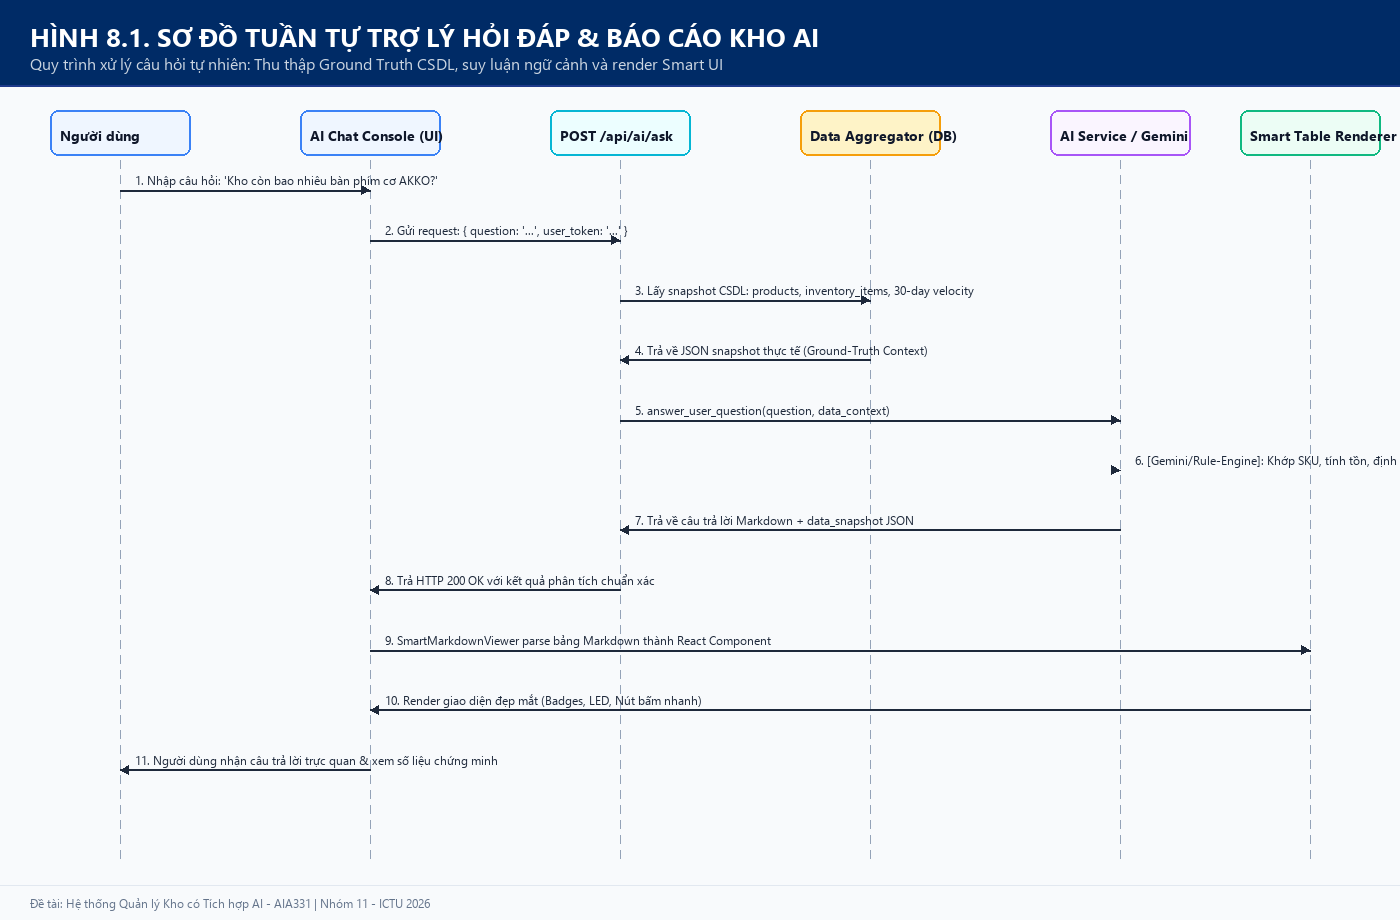
\includegraphics[width=0.92\textwidth]{figures/sequence_ai_report.png}
\caption{Sơ đồ tuần tự (Sequence Diagram) luồng xử lý câu hỏi của Trợ lý AI NLP}
\end{figure}

\section{Kỹ thuật Prompt Engineering và Grounding dữ liệu chống ảo giác}

Nhằm loại bỏ hoàn toàn hiện tượng 'ảo giác' (Hallucination) thường gặp ở các mô hình ngôn ngữ lớn, hệ thống áp dụng kỹ thuật Grounding dữ liệu nghiêm ngặt theo các nguyên tắc:

1. Chỉ cung cấp cho mô hình các dữ liệu JSON đã được truy vấn trực tiếp từ CSDL.

2. Thiết lập System Prompt bắt buộc: 'Chỉ trả lời câu hỏi dựa DUY NHẤT vào dữ liệu JSON kho hàng thực tế được cung cấp. Tuyệt đối không tự bịa đặt dữ liệu hay đưa ra số liệu không có trong ngữ cảnh.'

3. Đặt tham số nhiệt độ mô hình (Temperature) ở mức 0.2 để tối đa hóa tính tất định và chuẩn xác của câu trả lời.

\section{Cơ chế Fallback sang Rule Engine nội bộ}

Khi hệ thống chạy trong mạng nội bộ không có kết nối Internet hoặc khi API Key của nhà cung cấp LLM hết hạn ngạch ngắt kết nối, hệ thống sẽ bắt ngoại lệ một cách êm ái và tự động kích hoạt Rule-based Engine nội bộ viết hoàn toàn bằng Python.

Rule Engine đọc trực tiếp snapshot JSON để tính toán các bảng thống kê và sinh báo cáo có định dạng chuẩn xác, đảm bảo 100\% tính sẵn sàng của hệ thống trong mọi hoàn cảnh vận hành.

